\chapter{人工智能基础}
人工智能是一门旨在赋予机器模仿和实现人类智能行为的技术,涵盖从基础的逻辑推理到高度复杂的学习过程,广泛应用于各类智能化任务。随着技术的不断进步,机器学习和深度学习逐渐成为人工智能的核心驱动力,它们让人工智能从早期依赖人为设计规则的模式,迈向通过数据发现规律并自适应调整的全新阶段。这种从“规则驱动”到“数据驱动”的转变,使得人工智能能够应对更加复杂、多变的现实问题。本章将从人工智能、机器学习和深度学习之间的关系入手,引导读者逐步了解机器学习和深度学习的基础知识。

\section{人工智能、机器学习、深度学习的关系}

人工智能作为一个广泛的技术领域,其核心目标是赋予机器执行复杂任务的智能能力,包括理解语言、识别图像以及做出决策等。在实现这些能力的过程中,机器学习和深度学习发挥了至关重要的作用。如果将人工智能比作一个广袤的宇宙,那么机器学习便是其中一颗明亮的星球,而深度学习则是这颗星球上最璀璨的宝石。

人工智能的早期发展主要依赖于人为设计的规则和逻辑推理。然而,随着应用场景的复杂化和多变性,这种基于规则的方法逐渐显得捉襟见肘。为了应对复杂环境的挑战,人工智能的发展逐步转向数据驱动的机器学习。机器学习通过训练计算机在大量数据中发现模式,从而实现预测、分类等任务,而无需事先编写明确的规则。例如,在推荐系统中,机器学习模型能够通过分析用户的历史行为数据,预测用户可能感兴趣的内容。

在机器学习的框架之下,深度学习的引入进一步增强了人工智能的能力。深度学习模拟了人脑神经网络的结构,可以自动提取数据中的特征,减少了对手工特征工程的依赖。在图像处理任务中,深度学习通过多层神经网络自动学习图像中的边缘、形状以及更复杂的结构,从而实现高精度的图像识别。这种自动化的特征提取能力,使深度学习在处理语音、文本和图像等复杂数据时表现尤为出色。

深度学习技术的成功离不开现代硬件的支持,尤其是图形处理单元(GPU\footnote{图形处理单元(Graphics Processing Unit, GPU):一种专为并行计算设计的硬件设备,最初用于加速图形渲染任务,如游戏画面和3D建模。GPU拥有大量的小型计算核心,能够同时处理多个数据块的计算任务,这种特性使其在深度学习模型训练中发挥了重要作用,大幅提升了神经网络的计算速度和效率。})的普及起到了关键作用。与传统的中央处理单元(CPU\footnote{中央处理单元(Central Processing Unit, CPU):计算机的核心处理器,主要负责执行程序中的各种逻辑和运算任务。CPU更擅长处理单一的复杂任务,类似于一位精通多种技能的工匠,但其核心数量较少,因此在处理需要大量并行计算的任务时效率较低。})相比,GPU在处理深度学习任务时展现出了显著的优势。

深度学习的训练过程涉及大量矩阵运算\footnote{矩阵运算是指对二维数组(矩阵)进行的加法、乘法、转置等操作,在深度学习中广泛应用于神经网络的权重更新、激活函数计算等环节。这些运算本质上是线性代数的核心内容,支撑着模型的前向传播和反向传播过程。},这是一个典型的计算密集型过程。矩阵运算贯穿于神经网络的前向传播和反向传播阶段,包括对多个变量的加法、乘法以及权重更新等操作\footnote{矩阵运算是神经网络计算的基础。前向传播过程中,模型需要对输入数据与权重矩阵进行乘法运算,再加上偏置项,从而得到各层的输出结果。而在反向传播中,模型通过链式求导法则对误差进行传播,并根据梯度更新每一层的权重和偏置参数。矩阵的乘法和转置操作在权重更新的过程中尤为重要,影响了模型的收敛速度和精度。}。这些操作通过大量线性代数计算支撑起模型的训练过程,是深度学习的核心步骤。传统的CPU架构更适合逐步完成复杂计算任务,类似于一位经验丰富的工匠,能够独立、高效地处理精细的工作。然而,当面对大批量的简单、重复任务时,CPU的效率就显得捉襟见肘。相比之下,GPU(图形处理器)则凭借其并行计算能力,能够同时运行数百甚至数千个计算核心,处理多个数据点的运算任务,类似于一条高效的流水线,每个核心负责一个简单的计算单元。在深度学习模型的训练过程中,GPU的优势尤为显著。例如,在权重更新阶段,GPU可以同时更新网络中数千个神经元的参数,从而大幅缩短训练时间。对于大型神经网络而言,使用CPU可能需要几天甚至几周才能完成训练,而采用GPU往往能够将时间缩短至数小时或数天。这正是由于GPU拥有强大的并行计算能力,深度学习技术才能快速发展,推动解决比以往更为复杂和大规模的问题,并在图像识别、语音处理等领域取得了突破性进展。

总体而言,人工智能、机器学习和深度学习之间形成了一种紧密的层级关系。人工智能作为最终目标,旨在实现机器的智能化;机器学习则是实现这一目标的重要工具,而深度学习是机器学习中更强大、更灵活的实现方法。三者的协同发展推动着智能系统不断突破技术边界,变得更加高效和精准。在后续学习中,将进一步探讨机器学习和深度学习的核心原理及其具体应用场景。

\begin{figure}[H]
	\centering
	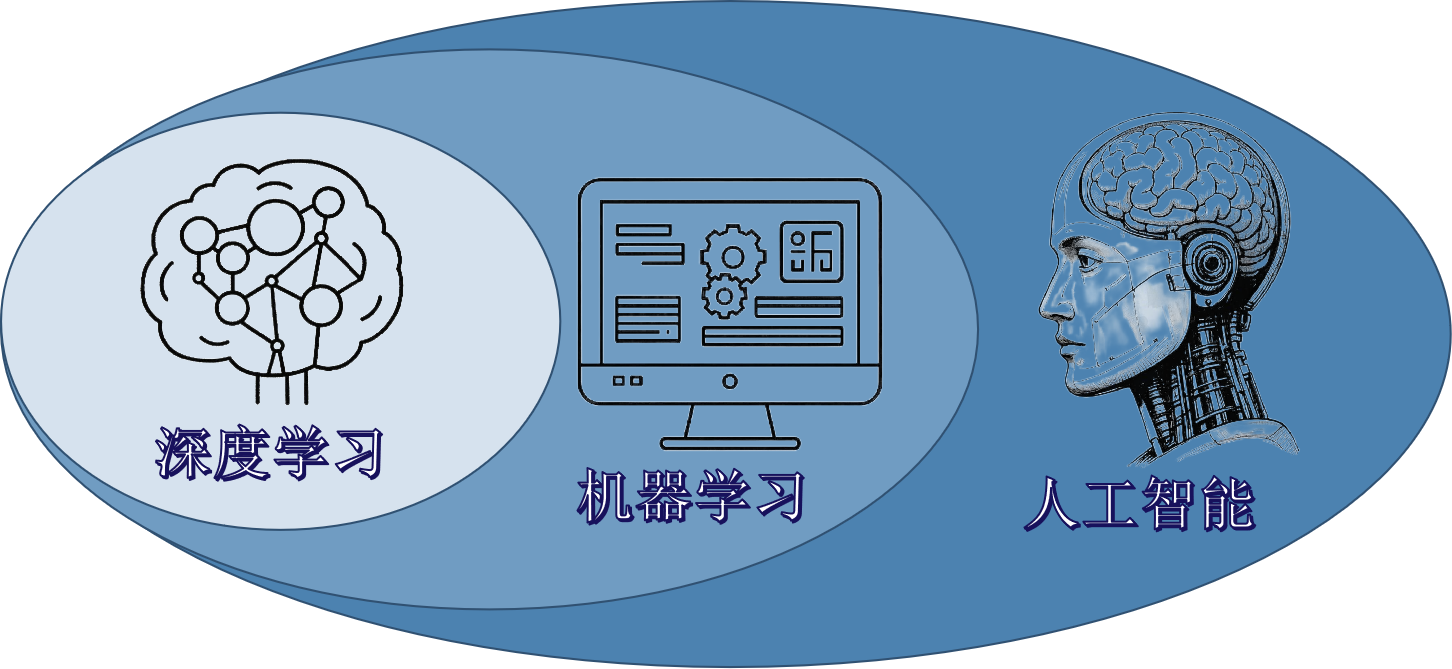
\includegraphics[width=0.9\linewidth]{image/2/人工智能、机器学习、深度学习.png}
	\caption{人工智能、机器学习、深度学习}
\end{figure}

\section{机器学习}

在上一小节中已经介绍了人工智能、机器学习和深度学习之间的关系。作为人工智能发展的核心支柱,机器学习使计算机能够在复杂多变的环境中实现“举一反三”,无需手动编写详尽的规则即可完成各种识别和预测任务。本章节将以入门的视角,探索机器学习的基本概念、核心流程,以及常见的算法与评估方式。通过引入“烘焙蛋糕”这一生活化的场景示例,帮助读者快速建立对机器学习的直观认识。

机器学习的关键优势在于其自适应能力。与传统编程方式不同,传统编程要求开发者针对每个可能的情况编写具体的指令,而机器学习通过从数据中学习并不断调整和优化算法,使计算机能够更高效地处理复杂任务。这种方式不仅提高了系统的灵活性和适应性,还极大地拓展了人工智能的应用场景。从图像和语音识别到自然语言处理和自动驾驶,机器学习已成为现代科技的核心驱动力。

这种自我学习和持续优化的能力,使人工智能系统能够不断进步,应对新的挑战和需求。不仅如此,机器学习还具备前瞻性,能够帮助系统预测未来的变化并主动调整应对策略。接下来的小节将重点探讨机器学习的定义、原理、分类,以及常用的学习方法和模型评估方式,深入解析这一技术如何赋予人工智能强大的智能能力。

\subsection{机器学习的定义}

日常生活中,人们常常依靠“经验”来解决问题。例如在烘焙蛋糕的过程中,最初可能并不知道每种配料的具体比例或烘焙时间,但通过多次尝试和观察,逐渐掌握了哪些步骤和调整能让蛋糕更加松软或香甜。这一过程无需从头到尾严格的步骤指导,而是依赖对配料变化、温度控制等因素的持续感知和总结,逐步形成新的烘焙策略。

机器学习的核心思想便是将这种“经验学习”的模式赋予计算机,使其能够模仿人类的学习过程。在传统编程方法中,需要事先为计算机设定详尽的规则,以应对各种具体场景。然而,许多实际问题难以通过显式指令解决。要让计算机学会制作不同类型的蛋糕,难以用固定的规则描述每种配料的变化和时间控制的精确步骤。与其手动编写这些复杂规则,不如让计算机“观察”大量烘焙案例的步骤和结果,通过试错和归纳自动找到制作成功蛋糕的关键特征。在完成训练后,计算机就能根据新的配方或烤箱条件调整烘焙策略,而无需额外更新规则或补充新指令。

从本质上讲,机器学习的核心在于将繁琐的规则制定过程转换为对数据的“经验学习”过程,让计算机能够在大规模、复杂环境中自主识别模式、归纳规律。通过已有数据和特定算法的结合,机器学习模型不断迭代和优化,使其在面对新场景时也能做出准确的判断或预测。这种方式不在于提供现成的答案,而是赋予计算机“学习”的能力,使其具备活学活用、举一反三的特性。同时,机器学习还能帮助挖掘数据中隐藏的内在逻辑与关联,从而形成更深层次的洞察。

随着数据规模的增长及维度和结构的复杂化,传统规则编程显得捉襟见肘。机器学习则通过分类、回归、聚类、降维\footnote{分类、回归、聚类和降维是机器学习中常用的四类方法。分类是将数据分配到不同类别的过程,例如垃圾邮件过滤;回归用于预测连续数值,例如房价预测;聚类是将数据划分为具有相似特征的组,例如客户分群;降维则是减少数据集中变量数量的方法,以降低计算复杂度并保留数据的关键信息。}等多种方法,对大规模、非线性数据\footnote{非线性数据是指变量之间的关系无法用简单的直线表达的复杂数据类型。}进行建模和模式识别,并在训练过程中不断修正假设与参数。这种基于数据的迭代学习\footnote{迭代学习是指通过反复调整模型和重新评估结果,逐步改进模型性能的过程。},使得计算机在处理复杂任务时能够灵活调整决策策略,展现出高度的适应性和智能化。因此,机器学习使计算机在没有明确指令的情况下,通过自我试验和归纳逐步成长为“智慧型助手”。它不仅能分担大量重复性、模式化的工作,还在持续推动各行业的技术变革。

\subsection{机器学习原理}

机器学习的运作原理大致可以分为几个关键环节:数据收集与整理、特征提取与选择、模型训练、验证与评估\footnote{这些步骤构成了机器学习模型的核心流程。数据收集与整理指的是获取和清洗数据,以确保数据的质量;特征提取与选择是从数据中识别和提取对模型预测有意义的变量;模型训练是利用算法调整模型参数,使其能够从数据中学习模式;验证与评估则是通过独立数据集测试模型的性能,确保模型在未见过的数据上也能有效应用。}以及持续改进。

数据是机器学习的基础材料\footnote{数据在机器学习中指可用于训练模型的信息集合,可能包含结构化数据(如表格)和非结构化数据(如图像、文本)。}无论是用于图像识别的像素值,还是用于文本分析的单词序列,数据的质量和数量直接影响模型的性能。为了确保模型的有效性,需要对收集到的数据进行清洗和整理,这一过程包括去除错误值、处理缺失数据、格式化数据类型等。数据清洗的目的是将原始数据转换为适合机器学习模型使用的结构化形式,从而避免模型受到噪声数据的干扰。清洗后的数据为模型的后续处理奠定了坚实的基础。

在清洗和整理完成后,需要对数据进行特征提取与选择\footnote{特征提取与选择是从数据中筛选出有助于模型预测的关键变量,以提高模型的准确性和效率。例如,从客户数据中提取年龄、收入等关键特征。}。特征是数据的核心信息载体,它们直接影响模型的预测能力。然而,原始数据中包含的大量信息并非都对模型有用,甚至可能导致模型性能下降。因此,特征选择的目标是识别出最具预测意义的变量,并剔除冗余或无关的信息。这一过程不仅能提高模型的训练效率,还能减少过拟合的风险。

在特征提取与选择完成后,模型进入训练阶段。模型训练\footnote{模型训练是指通过已有数据调整模型参数,使其能够识别数据模式并做出预测的过程,例如使用历史销售数据训练模型预测未来销量。}是机器学习的核心环节,旨在通过调整模型的参数,使其能够从数据中学习出隐藏的模式和规律。在训练过程中,模型不断对输入数据进行计算和分析,并根据设定的目标函数优化参数,从而提升其在训练数据上的表现。常见的训练方法包括监督学习、无监督学习和强化学习。监督学习通过带有标签的数据集进行训练,模型能够学习到输入数据与输出结果之间的映射关系;无监督学习则侧重于数据的内部结构分析,例如聚类和降维;而强化学习通过奖励机制引导模型的行为,使其在特定环境中优化决策。

在训练阶段完成后,模型需要通过验证与评估\footnote{验证与评估是指利用独立的数据集来测试模型性能,以衡量模型在处理新数据时的准确性和鲁棒性。}来测试其实际效果。验证的核心目的是衡量模型的泛化能力,即在未见过的数据上能否保持较高的预测准确率。常用的评估指标包括准确率、精确率、召回率和F1分数等,这些指标能够全面反映模型的预测性能。此外,还需要通过混淆矩阵等工具深入分析模型的分类错误情况,从而进一步优化模型。

在验证过程中,模型调优和参数调整也是不可或缺的环节。模型的调优通常包括调整超参数、选择合适的特征工程方法、尝试不同的算法架构等。这一过程需要结合开发者的经验和业务需求,通过不断试错来找到性能最佳的模型。调优后的模型通常具有更高的鲁棒性\footnote{鲁棒性指模型在面对噪声、异常数据或其他不可预见情况时,仍然能够保持稳定性能的能力。},即使在面对新环境或数据分布变化时,依然能够做出合理的预测。

整个机器学习流程是一个不断迭代的过程。在实际应用中,模型在部署后也需要持续监测和更新,以应对环境变化和数据分布的偏移。这种持续改进的过程,使得模型能够与时俱进,始终保持高效和准确的决策能力。这一过程展示了机器学习模型从数据中学习的核心逻辑。然而,要真正理解模型如何进行预测,还需要进一步探讨具体的算法。在机器学习的众多算法中,线性回归和逻辑回归是最基础且最常用的两种方法。它们不仅适用于广泛的实际场景,还为更复杂的模型提供了理论基础,接下来的学习将详细讨论这两种算法。

\section{线性回归与逻辑回归}

线性回归和逻辑回归是机器学习领域中两种基础且常用的模型,它们各自擅长解决不同类型的问题。可以将这两种模型类比为烘焙中的两大关键环节:线性回归用于分析原料的具体配比如何影响蛋糕的甜度或高度;逻辑回归则用来判断蛋糕是否符合质量标准。尽管名称相似,这两种模型在工作方式和应用场景上有着显著差异。

\subsection{线性回归}

线性回归是一种探索输入变量与输出变量之间线性关系的模型。它通过一条直线来描述数据点的趋势,进而实现对新数据的预测,如图\ref{fig:线性回归}所示。在线性回归的框架中,输入变量可以被看作是影响结果的因素,而输出变量则是最终的预测目标。

\begin{figure}[H]
    \centering
    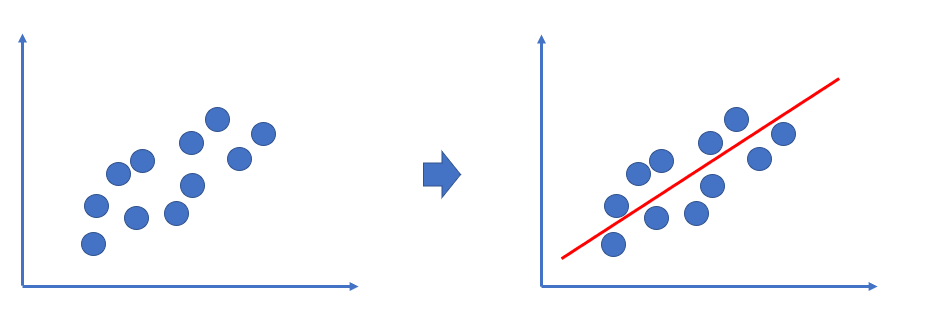
\includegraphics[width=0.8\linewidth]{image/2/线性回归.png}
    \caption{线性回归}
    \label{fig:线性回归}
\end{figure}
以烘焙为例,当试图研究糖的用量与蛋糕甜度之间的关系时,线性回归可以帮助找出两者的相关性。假设实验记录了几组数据:糖量为100克时,甜度评分为8分;糖量增加到150克时,甜度提升到10分;糖量进一步增至200克时,甜度达到12分。基于这些数据,线性回归模型可以生成如下公式:

\[
\text{甜度} = 0.02 \times \text{糖量} + 6
\]

该公式表明,糖量每增加1克,蛋糕的甜度将提升0.02分。如果目标是制作甜度评分为11分的蛋糕,可以反推出所需的糖量为175克。这样的预测过程展现了线性回归的核心功能:通过数据中的线性模式,准确估计连续变量的值。
线性回归的应用范围十分广泛,从房价预测到销售趋势分析,再到自然科学中的实验数据建模,这一模型以其直观性和高效性成为初学者的理想起点。

\paragraph{优点与局限}  

线性回归具有以下优点:它的原理清晰易懂,模型参数\footnote{模型参数是指模型中需要学习的系数,这些系数反映了每个输入变量对输出结果的影响大小。}可以直接反映输入变量对输出的影响,且计算效率较高,非常适合大规模数据集。然而,它也存在明显的局限性。例如,线性回归假设输入与输出之间存在线性关系,但许多现实问题是非线性的。此外,线性回归对数据中的异常值\footnote{异常值是指显著偏离其他数据点的值,可能由于测量误差或极端情况导致。在模型中,这些值会对结果产生较大影响,需加以处理。}敏感,这些异常值可能会显著偏离实际结果,从而影响模型的预测效果。

\subsection{逻辑回归}

逻辑回归是一种用于分类问题的模型,专注于解决“是或否”类型的问题。通过逻辑回归,可以根据输入特征预测某一对象属于特定类别的概率。

在电子邮件分类中,判断一封邮件是否为垃圾邮件是一个常见任务。某些记录显示,不同邮件特征对垃圾邮件识别的影响如下:包含“免费”关键词和多个链接的邮件通常被认为是垃圾邮件;而不包含这些特征的邮件则被认为是正常邮件。这些数据为逻辑回归模型提供了依据,帮助它计算特定邮件特征下邮件为垃圾邮件的概率。逻辑回归利用这些输入数据,通过拟合模型生成概率值。如果某封邮件的垃圾邮件概率为80\%,且这一概率高于设定的阈值\footnote{阈值是分类决策中的关键参数,用于将概率值划分为不同类别。合适的阈值选择需综合考虑分类任务的性质和错误成本。}(如50\%),那么模型将判定该邮件为“垃圾邮件”。反之,若垃圾邮件概率低于阈值,则判定为“正常邮件”。逻辑回归通过S型曲线\footnote{S型曲线(Sigmoid Curve)是一种数学函数形式:\( \sigma(x) = \frac{1}{1 + e^{-x}} \)。它能够将模型输入的线性结果平滑地映射到0到1之间,使得逻辑回归可以输出概率值,并实现分类判定。}将输入变量平滑映射到0到1之间,从而以概率形式输出结果(如图\ref{fig:逻辑回归}所示)。

\begin{figure}[H]
    \centering
    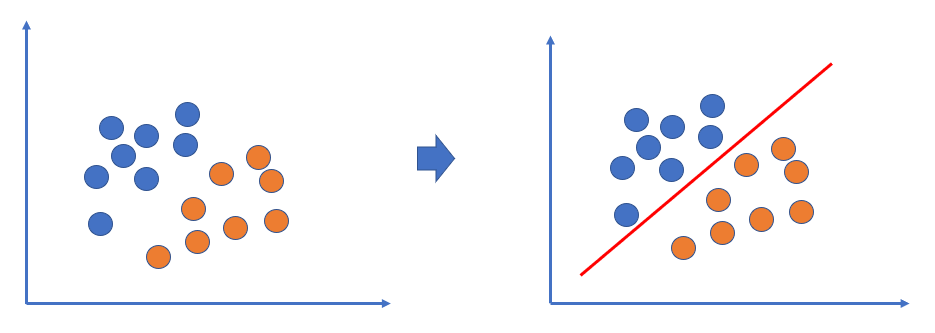
\includegraphics[width=0.8\linewidth]{image/2/逻辑回归.png}
    \caption{逻辑回归}
    \label{fig:逻辑回归}
\end{figure}

这种方法广泛应用于二分类任务,包括信用卡欺诈检测、疾病诊断预测以及电子商务中的用户行为分析等。

\paragraph{优点与局限}  

逻辑回归以其简洁和高效的算法,在分类任务中表现突出。它可以输出分类概率,直观反映模型的信心。然而,逻辑回归通常仅适用于二分类问题,多分类任务需通过Softmax回归\footnote{Softmax回归是一种扩展逻辑回归以支持多分类任务的方法。它使用Softmax函数将模型的输出映射到多个类别的概率分布上,从而实现对多个类别的预测。}等扩展方法来实现。此外,逻辑回归对输入变量的独立性假设较强,若输入变量之间存在显著相关性,模型的性能可能受到影响。


\subsubsection{线性回归与逻辑回归的对比}

尽管线性回归和逻辑回归在某些方面存在相似性,它们都属于回归模型,且都依赖输入变量与输出的关联性,但它们在目标、输出形式和应用场景上有着显著区别,如表\ref{table999}。

\begin{table}[H]
    \centering
    \caption{线性回归与逻辑回归的对比}
    \label{table999}
    \begin{tabular}{|p{2cm}|p{5cm}|p{5cm}|}
        \hline
        \textbf{特性} & \textbf{线性回归} & \textbf{逻辑回归} \\
        \hline
        \textbf{目标} & 预测连续数值(如甜度、高度) & 判断分类结果(如是否合格) \\
        \hline
        \textbf{输出形式} & 实数值(可为正或负) & 概率值(0到1之间) \\
        \hline
        \textbf{适用问题} & 连续值预测问题 & 分类问题(二分类为主) \\
        \hline
        \textbf{优势} & 简单直观,结果易解释,计算快速 & 概率输出,专注分类,计算高效 \\
        \hline
        \textbf{局限性} & 仅适用于线性关系,对异常值敏感 & 主要用于二分类,对多分类需调整 \\
        \hline
    \end{tabular}
\end{table}


\subsubsection{应用场景与选择}

在线性回归和逻辑回归的应用中,方法的选择通常依据任务的核心目标。如果需要预测具体数值,如蛋糕的甜度或高度,线性回归更加适用;而当任务需要判断类别归属,如蛋糕是否合格,逻辑回归则是更优的选择。在某些复杂场景中,这两种方法可以结合使用。通过线性回归预测蛋糕的具体特性,然后利用逻辑回归对预测结果进行分类,这种组合方式能够进一步提升分析能力和结果的准确性。

线性回归和逻辑回归作为机器学习领域的基础模型,其简单且高效的特性使其广泛应用于各种场景。掌握这两种模型的原理和应用,可以为后续学习更复杂的算法提供坚实的理论基础。

\subsection{评估与优化}

烘焙中的理想食谱并不能保证每次都能做出完美的蛋糕。火候、温度、配料比例等细节仍需调整,才能烘焙出最佳效果。同样,机器学习模型在训练完成后,也需要通过全面的评估与优化来提升性能,确保在处理新数据时依然能给出准确预测。这不仅是对模型效果的检验,更是提高模型泛化能力的关键步骤。评估与优化的过程,类似于不断完善烘焙技艺,以保证每一批蛋糕都达到预期标准。

\subsubsection{多角度评估模型表现}

\subsection{评估与优化}

评估模型的表现,不仅仅是简单地查看预测结果的准确性,而是需要从多个角度全面分析其能力,就如同品尝蛋糕时,不仅要关注其外观,还需要检查内部的口感和质地。单一的评估指标往往无法全面反映模型的优劣,因此需要多种评估标准相互结合。

准确率是最常用的评估指标,类似于蛋糕的外观评分,能够直观反映模型整体预测的正确性。例如,如果制作了100个蛋糕,其中90个符合标准,那么模型的准确率为90\%。然而,准确率可能掩盖模型在某些类别上的问题。例如,一个外观完美的蛋糕可能存在口感不佳的问题。同样,某些高准确率的模型可能在少数类别上的表现较差。

为了更深入了解模型的具体表现,精确率和召回率是两个重要的补充指标。精确率衡量的是模型预测为正类时的准确比例,比如预测出10个蛋糕合格,但实际上只有8个符合标准,则精确率为80\%。这一指标强调预测的精准性。相比之下,召回率关注的是模型对所有正类样本的覆盖能力,例如实际有10个合格蛋糕,而模型预测了其中8个,则召回率也是80\%。高召回率表明模型尽可能减少遗漏,确保所有符合标准的蛋糕都被检测出来。

精确率和召回率往往需要平衡,为此引入了F1分数作为综合评估标准。F1分数是精确率和召回率的调和平均值\footnote{调和平均值是一种统计学计算方法,强调小数值对整体结果的影响。公式为:\( F1 = 2 \times \frac{\text{精确率} \times \text{召回率}}{\text{精确率} + \text{召回率}} \)。它特别适用于评估需要在多个指标间找到平衡的场景。},能够反映模型在这两个维度上的综合表现。F1分数越高,意味着模型在预测准确性和覆盖能力之间达到了良好的平衡。

此外,AUC-ROC曲线提供了更全面的视角。AUC值(曲线下面积)衡量模型在不同阈值下区分正类和负类的能力,接近1的AUC值表示模型具有出色的区分能力。ROC曲线展示了假正率和真正率之间的关系\footnote{假正率(False Positive Rate, FPR)是指将负类误判为正类的比例,公式为:\( \text{FPR} = \frac{\text{假正例}}{\text{实际负类}} \)。真正率(True Positive Rate, TPR)是指正类被正确预测的比例,公式为:\( \text{TPR} = \frac{\text{真正例}}{\text{实际正类}} \)。这两个指标用来分析模型在不同预测阈值下的性能表现。},帮助发现模型在不同阈值下的表现。这一过程类似于不断调整烘焙时间和温度,试验不同参数组合,最终找到最佳烘焙方案。

\subsubsection{提升模型的泛化能力}

模型训练中的过拟合和欠拟合是两个常见问题,需要通过优化来解决。过拟合的模型虽然在训练数据上表现优异,但在新数据上效果较差,类似于烘焙师只会按照特定食材制作蛋糕,却无法适应不同的环境和材料。过拟合通常可以通过正则化\footnote{正则化是一种机器学习技术,旨在限制模型的复杂度,避免过度拟合训练数据。常见的正则化方法包括L1正则化(Lasso)和L2正则化(Ridge),通过在损失函数中加入惩罚项减少模型对特定特征的依赖。}技术、增加数据多样性或使用简化模型来缓解。

另一方面,欠拟合则是模型未能充分学习数据规律\footnote{数据规律指数据中隐藏的模式或趋势,模型需要通过训练过程识别这些规律来提高预测能力。未能识别数据规律可能是由于模型过于简单或数据不足导致的。}的表现,导致预测能力不足。欠拟合类似于烘焙师对制作工艺的了解不足,导致蛋糕无论外观还是口感都不理想。解决欠拟合的方法包括提高模型复杂度\footnote{模型复杂度是指模型的容量或表达能力,通常由参数的数量或模型结构的层次决定。较高的复杂度可以让模型更好地适应复杂的数据分布,但可能导致过拟合问题。}、增加训练数据或改进特征提取方式。

\subsubsection{超参数调整与优化}

模型的优化离不开超参数调整\footnote{超参数调整是指在模型训练之前手动或自动选择适合的参数,这些参数不会通过训练过程更新,例如学习率、正则化系数和批量大小。超参数调整直接影响模型的收敛速度和性能。}这一关键步骤,就如同调整烘焙温度和时间以适应不同季节的环境。超参数是模型训练前需要设置的参数,例如学习率\footnote{学习率是超参数之一,用于控制模型每次更新参数的步幅大小。较大的学习率可能导致模型跳过最优解,而较小的学习率则可能使训练过程过于缓慢。找到适当的学习率有助于平衡训练效率和准确性。}、正则化系数\footnote{正则化系数是超参数之一,用于控制正则化项对模型的约束力度。较大的正则化系数可以有效减少过拟合,但可能导致欠拟合。}和批量大小\footnote{批量大小是指每次训练过程中用于更新模型参数的数据样本数量。较大的批量大小可以提高计算效率,但可能影响模型的泛化能力;较小的批量大小通常需要更长的训练时间,但可能更有助于模型的泛化。},它们直接影响模型的训练过程。

学习率决定了每次模型更新的步幅。学习率过大可能导致模型跳过最佳解,而学习率过小则会使训练过程过于缓慢。找到合适的学习率对模型优化至关重要。常用的调整方法包括网格搜索\footnote{网格搜索是一种系统化的超参数调整方法,通过在预设的参数网格中逐一尝试每种组合,找到最优的超参数配置。}和随机搜索\footnote{随机搜索是一种超参数调整方法,通过在参数空间中随机采样组合,寻找性能最佳的超参数配置。相比网格搜索,随机搜索在高维参数空间中更高效。},这些方法通过系统化地探索不同的超参数组合,帮助找到最优解。

\subsubsection{错误分析与改进策略}

在模型优化过程中,错误分析\footnote{错误分析是通过检查模型预测错误的样本,分析模型性能问题的一种方法。它有助于发现模型设计或数据分布中的不足,从而为进一步优化提供指导。}是重要的诊断工具。通过检查模型预测错误的数据样本\footnote{样本是指用于模型训练或评估的单个数据点,例如一个记录、一张图片或一段文本。样本的质量和多样性对模型的性能有直接影响。},可以发现数据或模型设计中的不足。例如,某些类别的表现可能较差,这往往与数据不平衡\footnote{数据不平衡是指数据集中不同类别的样本数量分布不均,可能导致模型对样本数量较多的类别预测较好,而对样本较少的类别表现较差。}有关。此外,特征不足\footnote{特征不足指用于训练模型的输入特征未能充分描述数据中的规律,导致模型无法有效区分不同类别或预测目标。}或噪声干扰\footnote{噪声干扰是指数据中存在与预测目标无关或错误的部分信息,例如测量误差或标注错误。这些干扰会降低模型的学习能力和预测准确性。}也可能是造成问题的原因。

针对上述问题,可以通过增加数据样本数量以平衡数据分布、重新设计特征工程以丰富模型输入信息,或通过数据清洗减少噪声对模型的影响。此外,调整模型结构或引入正则化技术也有助于改善模型表现。

\subsubsection{持续优化与迭代改进}

模型优化是一个持续的迭代过程。每次训练、评估和调整后,都可能发现新的改进方向。类似于烘焙师不断尝试新配方和技术,机器学习模型也需要在实验中逐步完善。随着数据量的增加和算法的改进,模型的性能将逐渐提升,最终能够适应更广泛的应用场景。

评估与优化是模型开发中不可或缺的环节。通过全面评估、多维度分析、针对性优化和持续迭代,可以显著提升模型的准确性和稳定性,确保其在复杂任务中的可靠表现。

在机器学习的持续发展中,线性回归和逻辑回归奠定了预测与分类的基础。然而,面对更复杂的现实世界问题,传统的算法在处理大规模数据和复杂特征时存在一定局限。此时,深度学习应运而生,提供了一种强大且灵活的工具,通过模拟人类神经网络的方式处理数据,解决多样化的任务。接下来的内容将深入探讨深度学习的核心原理与技术,更全面地掌握这一技术在人工智能领域中的关键作用。

\section{深度学习}

深度学习是人工智能领域的重要分支,正以高速发展的势头在众多领域展现其潜力。从自动驾驶汽车到语音助手,从图像识别到自然语言处理,其应用场景广泛且深刻。然而,深度学习的复杂性常让人望而生畏:为何称其为“深度”?它与传统机器学习有何差异?通过多层结构,深度学习如何从数据中提取复杂的规律?接下来的学习将从深度学习的起源、核心原理到其快速发展的关键因素进行分析。通过通俗的比喻与清晰的阐述,逐步揭示深度学习的本质,帮助更全面地理解这一技术的强大能力及其面临的挑战。

\subsection{从“学习”到“深度学习”}

深度学习是一种模拟人类大脑学习方式的技术,通过多层结构\footnote{多层结构是指深度学习模型由多个隐藏层组成,每一层负责提取数据的不同特征,从简单到复杂逐步处理,从而解决复杂问题。例如,第一层可能提取图像的边缘信息,第二层识别形状,最后的层则判断具体的类别。}自动提取数据中的特征,用以解决复杂问题。这一技术的兴起可类比为园丁管理复杂花园的过程。

在传统花园管理中,园丁通常依赖书本或经验总结出的固定规则(例如“晴天需增加浇水量,雨天减少施肥”)进行管理。这种方法类似于传统机器学习,依靠预设的规则解决问题。然而,当环境变得复杂,例如连续暴雨导致土壤过湿,或病虫害突然爆发,固定规则往往难以应对。这时,深度学习展现出其独特的优势。通过多层结构逐步学习,深度学习能够从复杂数据中提取关键特征,灵活调整策略,从而更好地适应多变的条件,为园丁提供更高效的解决方案。

深度学习与传统方法的核心区别在于它引入了更灵活的自动化学习方式。通过构建多层神经网络\footnote{\textbf{神经网络}是一种仿生计算结构,模拟人脑的工作方式,由输入层、隐藏层和输出层组成。每一层通过权重和偏置连接,用于提取数据的特征和模式,最终形成预测或决策。},深度学习可以自动分析和综合多个变量,给出更精准的判断和策略。以花园管理为例,当土壤湿度数据被输入系统后,第一层神经网络判断是否存在干旱问题,第二层结合温度和光照强度评估植物的蒸腾速率,最终的输出层综合这些信息,给出“浇水3升”的具体方案。通过逐层处理的机制,深度学习能够高效处理复杂的多变量决策问题,显著提升管理效果。

总体而言,深度学习的多层结构和自动学习能力摆脱了传统方法对固定规则的依赖。这种灵活性不仅让深度学习在园艺管理这样的场景中表现优越,更使其在图像、语音、文本等复杂领域中具有广泛的应用价值。

\subsection{深度学习和机器学习的区别}

深度学习与传统机器学习的区别主要体现在对规则的依赖程度上。传统机器学习通常依赖人为制定的规则,例如设定具体的浇水或施肥条件。而深度学习则通过对大量数据的训练,自主学习规律,无需人为干预。传统机器学习可以类比为为园丁准备了一本详细的说明书,上面标明“土壤湿度低于20\%时浇水”。这种方法在简单场景下效果良好,但在环境复杂且多变时可能失效。

相比之下,深度学习通过观察大量花园的历史数据(例如土壤湿度、天气、植物生长状态),能够从中自动发现隐含规律。例如,深度学习可能会发现“在持续高温条件下,即使湿度高于20\%,植物仍需额外浇水”,并据此调整策略。

设想一个园丁记录了一年的浇水数据,包括土壤湿度、温度、光照和植物的生长状态。传统机器学习只能基于已设定的条件进行判断,例如“湿度低于某个阈值时浇水”。而深度学习系统则能够从这些数据中提取更深层次的规律,如“高温条件下需更频繁浇水”,或者“某些植物品种对湿度的变化更敏感”。这种能力使深度学习在面对复杂问题时更加高效和灵活。
    
\subsection{深度学习的崛起}

深度学习的崛起得益于数据的爆发性增长、计算能力的提升以及算法的改进。

\subsubsection{数据的爆发}

随着现代技术的快速发展,数据的收集与存储变得更加便捷。从实时监控土壤湿度到记录光照变化,深度学习能够利用这些海量数据提取有价值的信息,为复杂问题的解决提供支持。例如,通过传感器\footnote{\textbf{传感器}:用于监测环境条件(如温湿度、光照强度等)的设备,能够实时采集数据,为分析和决策提供基础支持。},园丁可以记录一整年中植物在不同天气条件下的生长数据,从而为深度学习模型提供丰富的学习素材。

这些传感器不仅能够精准监控湿度和光照,还可以检测病虫害的早期迹象,为数据分析带来更大的广度和深度。随着数据量的不断积累,深度学习模型能够从中提取复杂的规律,灵活应对多变的环境条件。这种对数据的充分利用,使得深度学习在园艺管理等领域的应用具有更高的精准度和可靠性。


\subsubsection{计算能力的提升}
高性能计算设备(如GPU\footnote{\textbf{GPU}:图形处理单元,一种擅长并行计算的硬件,加速了深度学习中的大规模矩阵运算。})显著提升了深度学习的训练效率。对于一个大型花园的管理,传统计算可能需要数周才能完成分析,而使用并行计算的设备可以在数小时内完成。

\subsubsection{算法的改进}
卷积神经网络(CNN\footnote{\textbf{卷积神经网络(CNN)}:一种特别适合图像处理的深度学习模型,通过提取图像的局部特征进行分类和识别。})和循环神经网络(RNN\footnote{\textbf{循环神经网络(RNN)}:一种擅长处理时间序列数据的深度学习模型,可捕捉数据间的上下文信息。})等算法的进步,使深度学习在图像和时间序列任务中表现出色。

\subsection{深度学习的灵感来源}

深度学习的灵感来源于人类大脑的神经网络。大脑通过神经元的连接与协作完成信息处理,人工神经网络模仿了这一机制。

% \subsubsection{神经网络的分层结构}

% \begin{figure}
%     \centering
%     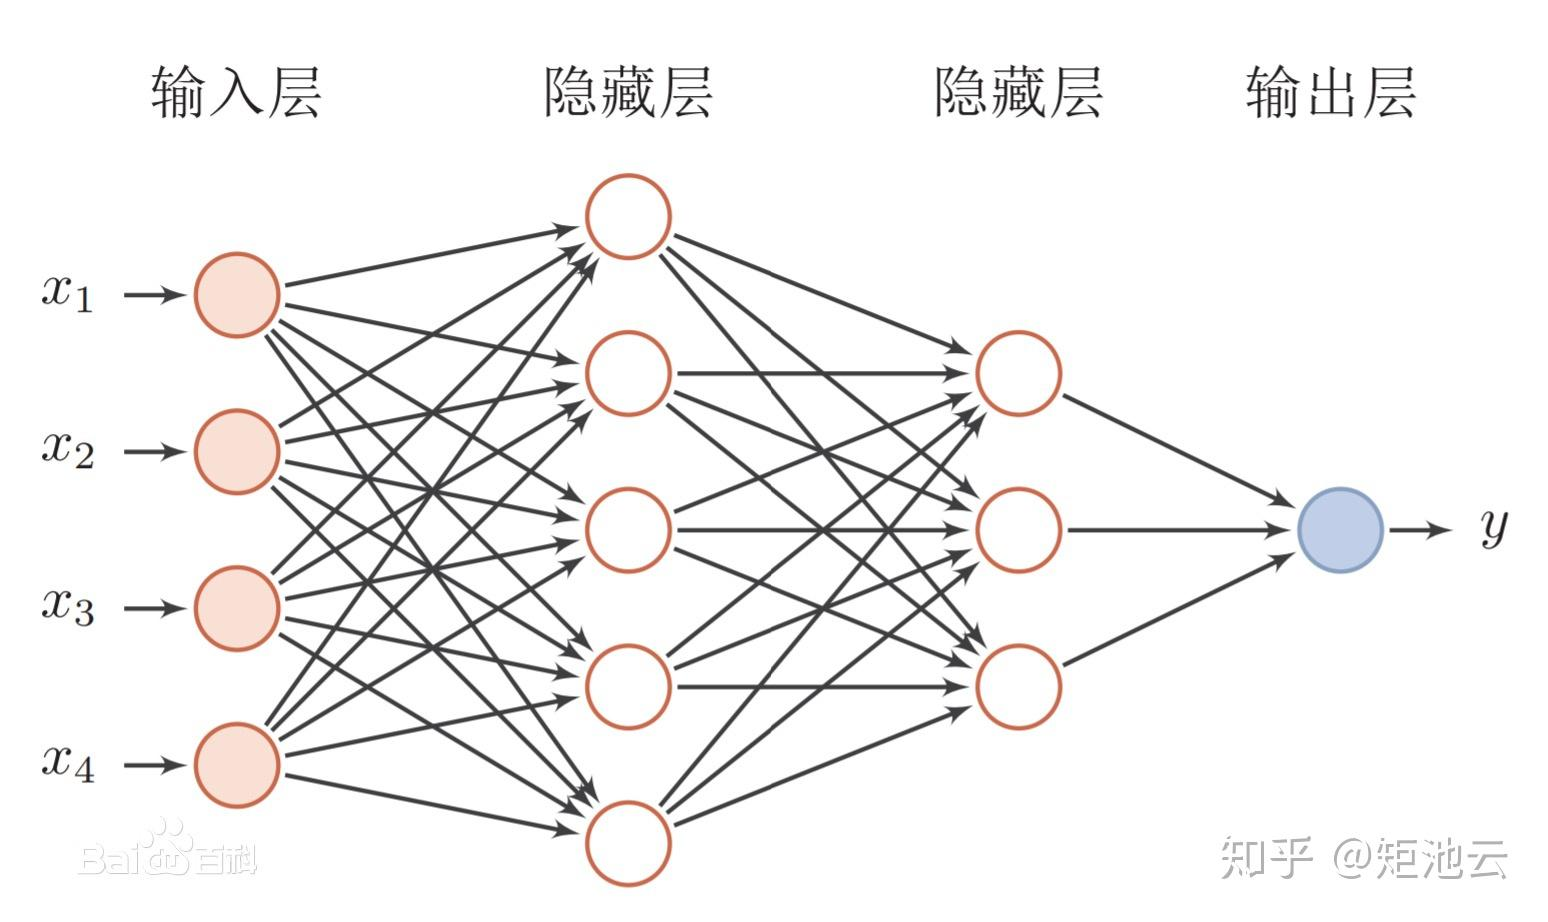
\includegraphics[width=0.8\linewidth]{image/2/神经网络层次结构.jpg}
%     \caption{神经网络层次结构}
%     \label{fig:神经网络层次结构}
% \end{figure}

人工神经网络由输入层、隐藏层和输出层组成,
% 如图\ref{fig:神经网络层次结构},
通过分层处理的方式,逐步将原始数据转化为有用的信息,最终完成复杂的任务。这种结构可以被理解为一个协作流程,其中每一层都有明确的职责。

\begin{itemize}
    \item \textbf{输入层}:负责接收和传递外部数据,例如数值、文本或图像等原始信息。输入层本身不对数据进行处理,只是将其传递给后续的隐藏层。
    \item \textbf{隐藏层}:是神经网络中处理和提取特征的核心部分。隐藏层通过权重和偏置的计算,对输入数据逐步加工,提取出不同层次的特征。浅层隐藏层通常提取数据的简单特征,例如边缘或基础模式,而深层隐藏层会捕捉更加抽象和复杂的特征,如关系模式或全局信息。
    \item \textbf{输出层}:负责根据隐藏层提取的特征生成最终结果。输出层的形式取决于具体任务,例如分类任务的输出层会提供类别概率,回归任务的输出层则会输出连续值。
\end{itemize}
以园丁的日常任务为例,当需要判断植物是否需要浇水时,神经网络的输入层会接收到土壤湿度和天气信息。隐藏层逐步分析数据,判断湿度是否充足、天气是否炎热以及植物当前的状态是否需要额外浇水。输出层则综合前面的分析结果,给出具体行动方案,如“浇水2升”或“无需浇水”。

神经网络的分层结构赋予其强大的适应能力。通过逐层处理,复杂的问题可以被分解成更小的任务,最终形成全面的解决方案。这种机制不仅提升了模型的分析能力,也使其能够应对多变的环境和动态数据。

\subsection{深度学习的三大核心层}

\begin{figure}[H]
    \centering
    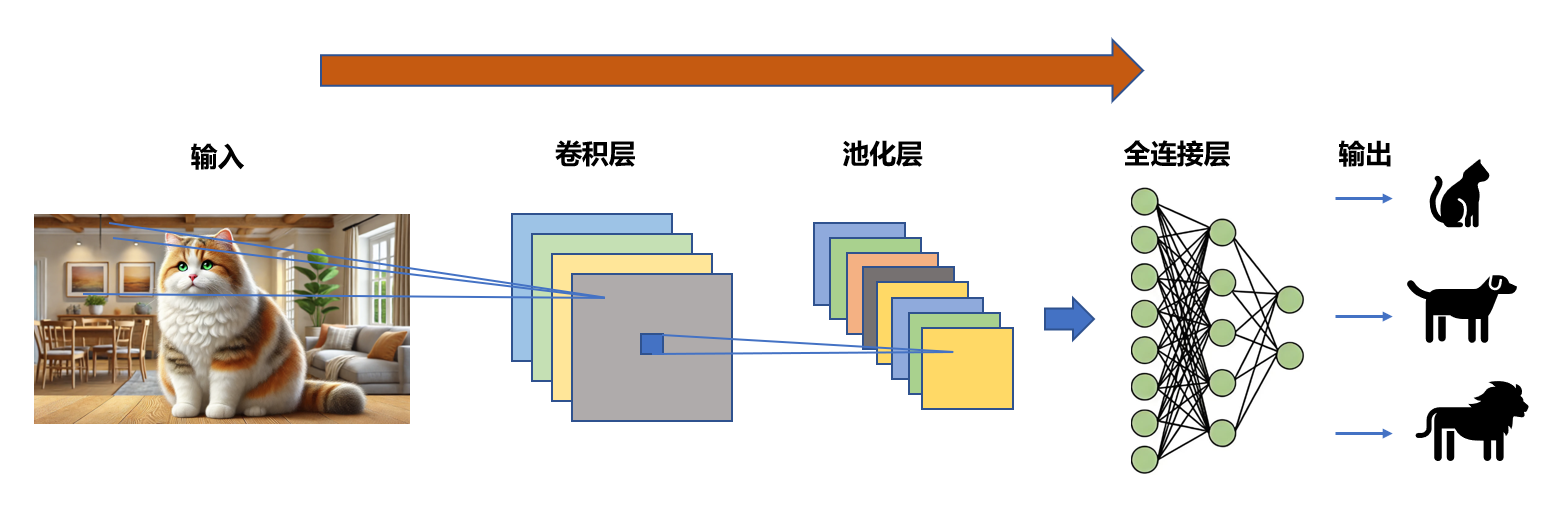
\includegraphics[width=\linewidth]{image/2/3大层.png}
    \caption{三大核心层}
    \label{fig:三大核心层}
\end{figure}

深度学习模型的分层结构是其强大性能的关键,不同的层负责处理数据的不同方面,逐层提取有意义的特征,最终实现复杂任务的解决。根据功能,深度学习的三大核心层包括卷积层、池化层和全连接层,如图\ref{fig:三大核心层}。接下来的学习将分别介绍这三种核心层的结构与作用,以帮助理解深度学习模型的工作原理。

\subsubsection{卷积层}

卷积层是深度学习模型的第一步,用于从数据中提取局部特征。它尤其适合处理具有空间结构的数据,例如图像或语音信号\footnote{\textbf{空间结构}是指数据中存在的内在规律,例如图像的像素分布或声音的时间序列。卷积层通过捕捉这些规律来提取有用信息。}。

卷积层的核心是“滤波器”\footnote{\textbf{滤波器}(Filter)是一种用于特征提取的小矩阵,也称为卷积核(Kernel)。它通过滑动窗口的方式与输入数据进行数学运算,提取局部特征,如图像的边缘、角点等。},它会像扫描仪一样滑动输入数据的不同区域,逐步识别局部特征。例如,在一张植物叶片的图片中,卷积层的第一步可能识别叶片的边缘,接着提取出叶片的纹理信息,最终提取整个叶片的形状。这种从局部到整体的逐步提取过程,使得卷积层能够自动学习图像中的模式。

卷积层具有两个显著特点:参数共享和局部连接。参数共享意味着同一个滤波器会应用于整个图像,减少了模型的参数数量;局部连接则使得卷积层仅关注局部区域,避免处理无关信息。这些特点使得卷积层既高效又适合处理大规模数据。

\subsubsection{池化层}

池化层的作用是简化数据,降低计算复杂度,同时提高模型对噪声\footnote{\textbf{噪声}是指数据中无关或随机的干扰,例如图像中的光照变化或语音中的背景噪音。池化层通过压缩数据,可以有效减少噪声对模型的影响。}的容忍能力。可以将池化层理解为数据的“压缩工具”,它从提取到的特征中保留最重要的信息,同时丢弃冗余内容。

池化的方式通常包括最大池化(Max Pooling)和平均池化(Average Pooling)。最大池化在一个小区域内选取最大值,类似于从一片区域中挑选最茂盛的植物;而平均池化则计算区域内所有值的平均数,更适合平滑数据。

池化层在图像处理中非常重要。例如,在识别一张花朵的图片时,池化层会将高分辨率的图片缩小,同时保留花朵的主要特征,例如形状和颜色。这种处理方式不仅减少了计算量,还能避免模型因过于关注细节而对噪声过敏。

\subsubsection{全连接层}

全连接层是神经网络的最后一步,它的任务是将前面层提取的特征整合起来,给出最终的结果\footnote{\textbf{结果}通常是分类或预测任务的输出,例如图像分类中的类别标签或回归问题中的预测值。}。可以将全连接层看作“决策者”,根据隐藏层提取的信息作出综合判断。

全连接层的结构特点是:每个节点\footnote{\textbf{节点}是神经网络中的基本单元,它接收输入、执行计算并输出结果,类似于生物神经元的功能。}与上一层的所有节点相连。这种完全连接的方式让全连接层能够综合所有信息,对输入数据进行全局分析。例如,在手写数字识别中,全连接层会结合卷积层和池化层提取的特征(如笔画方向、数字形状等),判断图片上的数字是“3”还是“8”。

全连接层虽然功能强大,但由于参数数量较多,容易导致过拟合\footnote{\textbf{过拟合}是指模型在训练数据上表现很好,但在新数据上效果较差的现象。通常可以通过正则化技术或增加数据量来缓解。}问题。因此,通常会使用正则化技术(例如Dropout\footnote{\textbf{Dropout}是一种正则化方法,通过随机丢弃部分节点,降低模型对特定特征的依赖,从而提高模型的泛化能力。})来减轻这一问题。

深度学习的三大核心层各自承担不同的功能,卷积层负责特征提取,池化层用于简化和压缩数据,而全连接层则负责整合信息并给出最终决策。三者的有机结合,使得深度学习模型能够高效地处理图像、语音和文本等复杂数据。

\subsection{深度学习的优势与挑战}

尽管深度学习在众多领域展现了其强大的能力,但也面临着数据依赖、计算资源需求和不可解释性等问题。

\subsubsection{数据依赖}
深度学习高度依赖数据的数量和质量。如果数据不足或分布不均,模型的性能可能大幅下降。例如,如果园丁的训练数据中仅包含晴天的条件,系统可能无法准确应对连续降雨的情况。多样化且高质量的数据是提升模型能力的关键。

\subsubsection{计算资源需求}
深度学习的训练需要强大的计算能力。例如,一个大型花园的管理系统可能需要处理上万条数据记录,如果没有高效的计算资源,训练过程可能耗时过长。优化硬件配置和算法设计是应对这一问题的主要方向。

\subsubsection{不可解释性}
深度学习的决策过程常被视为“黑箱”,即难以明确解释其具体判断依据。例如,一个植物养护模型可能建议“减少施肥量”,但无法具体说明原因。这种不可解释性限制了深度学习在某些高风险领域的应用。


\section{总结}

通过前面的学习,已经清晰地梳理了人工智能、机器学习和深度学习之间的关系,并深入探讨了它们的核心原理、模型特点和实际应用。从整体上来看,人工智能是一个宏大的技术目标,致力于赋予机器以类人智能,使其能够完成复杂的任务。而机器学习作为实现这一目标的重要工具,通过对数据的模式学习,使计算机具备自适应能力,完成分类、预测等任务。深度学习则作为机器学习中的重要分支,通过多层神经网络的特性,进一步增强了对高维、复杂数据的处理能力,推动人工智能技术在图像识别、语音处理和自然语言理解等领域取得了革命性的突破。

机器学习的核心优势在于其灵活性和强大的数据适应能力。通过分类、回归、聚类等方法,机器学习能够从海量数据中提取规律,为解决实际问题提供精准的工具。然而,面对复杂的非线性问题,机器学习传统方法的局限性逐渐显现。深度学习的出现,以其自动化的特征提取能力,解决了许多需要手工设计特征的问题,大幅提升了模型的性能。通过卷积层、池化层和全连接层的有机结合,深度学习不仅能够高效处理图像、语音和文本数据,还展现了对复杂任务的出色解决能力。

尽管深度学习具备强大的功能,但其面临的一些挑战不容忽视。例如,对海量数据和计算资源的依赖、高昂的训练成本,以及模型的不可解释性,都是当前研究者和从业者需要重点解决的问题。此外,如何将深度学习技术扩展到更多领域,以及实现模型在高效性和精准性之间的平衡,也是未来技术发展的关键方向。

人工智能、机器学习和深度学习的发展相辅相成,它们不仅为科学研究和工业生产带来了深远的影响,也在教育、医疗、金融等领域推动了创新和变革。未来,随着数据规模的进一步增长、计算能力的持续提升,以及算法的不断优化,人工智能技术将进一步拓展其应用场景,为人类社会带来更多可能性。

通过对人工智能基础知识的学习和理解,建立了一个坚实的理论基础,接下来的内容将继续聚焦更复杂的算法和技术应用,帮助全面深入地掌握人工智能技术的全貌,并探索其在实际问题中的应用潜力。

\section* {习题}

\subsection*{1. 烘焙师与人工智能的对比}
假设你是一名烘焙师,想要烘焙出最美味的蛋糕。你有两种方法可以选择:
\begin{itemize}
    \item 方法一:通过经验积累,记录每次烘焙的温度、时间、配料比例,并总结出最佳的配方。
    \item 方法二:你雇了一名助手,让他通过观察你的每次烘焙过程,自主总结经验,并在下一次尝试中做出更好的蛋糕。
\end{itemize}

\textbf{请回答:}
\begin{enumerate}
    \item 这两种方法分别对应人工智能中的哪两种学习方式?
    \item 为什么第二种方法(助手自主学习)更像深度学习?
    \item 你认为在现实生活中,人工智能助手会有哪些实际应用场景?
\end{enumerate}

\textbf{答案:}
\begin{itemize}
    \item 方法一是基于规则的传统编程或机器学习。
    \item 方法二更像深度学习,因为助手通过大量观察和实践,不断改进。
    \item 实际应用场景包括语音助手、自动驾驶、推荐系统等。
\end{itemize}

\subsection*{2. 自动驾驶汽车的“眼睛”}
自动驾驶汽车需要识别道路上的车辆、行人、交通信号灯等信息,以做出安全的驾驶决策。如果你是这辆车的设计师,你会面临以下挑战:

\textbf{请回答:}
\begin{enumerate}
    \item 如何让汽车“看清”周围的环境?
    \item 遇到大雾、暴雨等天气时,汽车识别路况的准确率会下降。你有什么改进方案?
    \item 汽车如何通过“学习”来提高在不同天气、不同路况下的表现?
\end{enumerate}

\textbf{答案:}
\begin{itemize}
    \item 使用摄像头和传感器作为“眼睛”。
    \item 数据增强技术(增加各种天气场景的数据)。
    \item 不断收集实际驾驶数据,优化深度学习模型,让汽车能适应更多环境。
\end{itemize}

\subsection*{3. 人工智能为什么需要“喂数据”?}
人工智能的学习过程就像一个新手园丁管理花园,他需要不断观察和记录花园的变化,才能找到最好的养护策略。

\textbf{请回答:}
\begin{enumerate}
    \item 如果园丁没有足够的数据,他能学会如何管理花园吗?为什么?
    \item 为什么深度学习需要大量的高质量数据?
    \item 你认为在哪些场景中,数据不足会导致人工智能模型表现不好?
\end{enumerate}

\textbf{答案:}
\begin{itemize}
    \item 如果没有足够的数据,园丁无法识别出所有情况,学习效果会很差。
    \item 深度学习依靠数据提取特征,如果数据不足或质量不好,模型无法准确学习。
    \item 医疗诊断、语音识别、自动驾驶等领域,数据不足可能导致错误判断。
\end{itemize}

\subsection*{4. 人工智能如何给你推荐电影?}
你在视频网站上看电影时,系统会自动推荐你可能喜欢的影片。

\textbf{请回答:}
\begin{enumerate}
    \item 系统是如何知道你喜欢哪类电影的?
    \item 如果系统总是推荐你不感兴趣的内容,你认为问题出在哪?
    \item 如果你是这个推荐系统的开发者,你会如何改进?
\end{enumerate}

\textbf{参考答案:}
\begin{itemize}
    \item 系统通过分析用户的观看历史、评分等数据,预测用户的偏好。
    \item 问题可能出在数据不足或推荐算法不准确。
    \item 改进方法包括收集更多用户行为数据、优化算法、增加用户反馈机制等。
\end{itemize}

\subsection*{5. 人工智能的偏见从哪里来?}
假设某公司开发了一款自动招聘系统,但后来发现它对女性求职者的评分普遍偏低。

\textbf{请回答:}
\begin{enumerate}
    \item 为什么人工智能系统会出现这种偏见?
    \item 如果你是系统的开发者,你会如何解决这个问题?
    \item 你认为人工智能的公平性重要吗?为什么?
\end{enumerate}

\textbf{参考答案:}
\begin{itemize}
    \item 人工智能系统的偏见可能来源于训练数据本身的偏见。
    \item 解决方法包括使用更公平的数据集、调整模型的评估标准等。
    \item 公平性很重要,因为人工智能的决策会直接影响人们的生活和工作。
\end{itemize}

\subsection*{6. 为什么图片识别这么“难”?}
人类能轻松识别图片中的猫和狗,但对计算机来说,这并不容易。

\textbf{请回答:}
\begin{enumerate}
    \item 计算机如何“看”一张图片?
    \item 为什么深度学习比传统方法更擅长识别图片?
    \item 你认为未来图片识别技术还可以在哪些领域应用?
\end{enumerate}

\textbf{参考答案:}
\begin{itemize}
    \item 计算机将图片转化为像素矩阵进行处理。
    \item 深度学习的卷积神经网络(CNN)能够自动提取图片中的关键特征。
    \item 可以应用于自动驾驶、医疗影像分析、安防监控等领域。
\end{itemize}

\subsection*{7. 人工智能如何不断“进步”?}
人工智能模型并不是一成不变的。它需要不断学习新的数据、应对新的挑战。

\textbf{请回答:}
\begin{enumerate}
    \item 为什么人工智能需要持续学习?
    \item 如果人工智能学到的“知识”过时了,会出现什么问题?
    \item 你认为人工智能的持续学习能力在现实生活中有什么重要意义?
\end{enumerate}

\textbf{参考答案:}
\begin{itemize}
    \item 人工智能需要持续学习来适应新环境、新数据。
    \item 如果知识过时,人工智能可能会做出错误的判断或决策。
    \item 持续学习能力在医疗、金融、教育等领域尤为重要,可以提高系统的准确性和实用性。
\end{itemize}

\subsection*{8. 深度学习和大脑的“学习”有何异同?}
深度学习的灵感来源于人类大脑的神经网络。

\textbf{请回答:}
\begin{enumerate}
    \item 人脑如何处理信息?
    \item 深度学习的神经网络如何模仿大脑?
    \item 你认为未来的人工智能会发展出类似人类的“思考”能力吗?为什么?
\end{enumerate}

\textbf{参考答案:}
\begin{itemize}
    \item 人脑通过神经元之间的连接和信号传递处理信息。
    \item 深度学习的神经网络通过多层神经元进行数据处理和决策。
    \item 未来人工智能可能会具备一定的“思考”能力,但它们的决策机制与人类不同。
\end{itemize}

\subsection*{9. 人工智能能预测天气吗?}
人工智能可以通过学习大量的天气数据来预测未来的天气情况。

\textbf{请回答:}
\begin{enumerate}
    \item 人工智能是如何根据历史数据预测未来的天气的?
    \item 如果出现极端天气,人工智能的预测准确性会受到影响吗?为什么?
    \item 你认为人工智能预测天气还有哪些应用场景?
\end{enumerate}

\textbf{参考答案:}
\begin{itemize}
    \item 人工智能通过分析历史数据中的模式,预测未来的天气变化。
    \item 极端天气可能会超出训练数据的范围,影响预测准确性。
    \item 可以应用于农业管理、自然灾害预警等。
\end{itemize}

\subsection*{10. 人工智能能帮助医生诊断疾病吗?}
医疗领域已经开始应用人工智能来辅助医生进行诊断。

\textbf{请回答:}
\begin{enumerate}
    \item 人工智能如何分析医疗影像来帮助医生诊断疾病?
    \item 人工智能诊断的结果可靠吗?为什么?
    \item 你认为人工智能在医疗领域的应用有哪些优势和挑战?
\end{enumerate}

\textbf{参考答案:}
\begin{itemize}
    \item 人工智能通过深度学习模型分析医疗影像,提取关键特征。
    \item 诊断结果的可靠性取决于模型的训练数据和算法的准确性。
    \item 优势包括提高诊断效率、减少误诊,挑战包括数据隐私和伦理问题。
\end{itemize}
